\documentclass{beamer}
\usepackage[absolute,overlay]{textpos}
\usepackage{graphicx}
\usepackage{subfig}
\usepackage{lmodern}   
\usepackage{multirow}
\usepackage{amsmath}
\usepackage{hyperref}
\usepackage{lineno}
\usepackage{adjustbox}

\usepackage{algorithm,algpseudocode}

\algdef{SE}[DOWHILE]{Do}{doWhile}{\algorithmicdo}[1]{\algorithmicwhile\ #1}%
\algnewcommand{\var}{\textit}

\hypersetup{
    citecolor=blue,
}

\definecolor{DiCITSBlue}{RGB}{59,83,145} 


\defbeamertemplate*{footline}{myfootline}
{
  \leavevmode%
  \hbox{%
  \begin{beamercolorbox}[wd=.333333\paperwidth,ht=2.25ex,dp=1ex,center]{author in head/foot}%
    \usebeamerfont{author in head/foot}\insertshortauthor
  \end{beamercolorbox}%
  \begin{beamercolorbox}[wd=.333333\paperwidth,ht=2.25ex,dp=1ex,center]{title in head/foot}%
    \usebeamerfont{title in head/foot}\insertshorttitle
  \end{beamercolorbox}%
  \begin{beamercolorbox}[wd=.333333\paperwidth,ht=2.25ex,dp=1ex,right]{author in head/foot}
    \usebeamerfont{date in head/foot}\insertshortdate{}\hspace*{2em}
    \insertframenumber{} / %\inserttotalframenumber\hspace*{2ex} 
    51\hspace*{2ex} 
%    \insertframenumber{}\hspace*{2ex} 
  \end{beamercolorbox}}%
  \vskip0pt%
}


\mode<presentation>
{
  \usetheme{Berlin}      % or try Darmstadt, Madrid, Warsaw, ...
  
  %\setbeamercovered{transparent}
   \setbeamercolor{structure}{fg=DiCITSBlue,bg=white}%yellow!40!red,bg=white}
   \setbeamertemplate{footline}[myfootline]
  
} 



\usepackage[english]{babel}
\usepackage[utf8x]{inputenc}


\title[Global Models]{Global Models for Time series Forecasting}
\author[Kasun Bandara]{\textbf{Google Cloud, Machine Learning Group} \and \\ \footnotesize September 01, 2021
\and \\\vspace{3mm} \textbf{\scriptsize Presenter} \and \\\vspace{2mm} Kasun Bandara
}
\institute{School of Computing and Information Systems \\\vspace{1mm} Melbourne Centre For Data Science \\\vspace{1mm} University of Melbourne}
\date[September 01, 2021]{}



\begin{document}
\begin{frame}[plain]
  \titlepage
\end{frame}

\begin{frame}{About Me}
\begin{itemize}
\item 2015 Graduated in Computer Science from University of Colombo School of Computing, Sri Lanka
\item 2015 Joined WSO2 Inc. as a Software Engineer
\item 2016-2020 Ph.D. in Computer Science, Monash University, Australia
 \begin{itemize}
  \item Topic: Forecasting In Big Data With Recurrent Neural Networks
  \item Machine Learning for Time Series Forecasting
  \item Research Internship at Walmart Labs, San Francisco, USA
  \item Research Scientist at Turning Point, Melbourne, Australia
  \item Data Science Tutor, Faculty of IT, Monash University
 \end{itemize}
\item 2021 Research Fellow, Melbourne Centre For Data Science, University of Melbourne
\end{itemize}
\end{frame}

\begin{frame}{About Me (2)}
\begin{itemize}
\item Research Interests
\begin{itemize}
 \item Global Forecasting Models
  \item Hierarchical Forecasting
  \item Retail sales/demand forecasting
  \item Demand forecasting (Retail, Energy, Health-care)
  \end{itemize}
\item Competition Fanatic
  \begin{itemize}
  \item Fuzz-IEEE Competition on Explainable Energy Prediction (\textbf{2nd Place})
  \item M5 Forecasting Competition (\textbf{Gold Medalist; World Rank 17/5500, Australia Rank 2nd})
  \item IEEE CIS Energy Forecasting Competition (\textbf{World Rank 4/100, Australia Rank 1st})
  \item Air-Liquide Energy Forecasting Competition (\textbf{World Rank 4/350, Australia Rank 1st})
  \item ANZ Customer Segmentation Challenge (\textbf{Top Performer})
  \end{itemize}
\end{itemize}
\end{frame}

%\begin{frame}{Monash MLTS: Overall Aims}
%\begin{itemize}
%\item Developing novel machine learning approaches (mainly deep learning based) for time series forecasting.
%\vspace{4mm}
%\item Forecasting applications to tackle real-world forecasting challenges.
%\vspace{4mm}
%\item Leveraging deep neural networks on large scales of related time series.
%\begin{itemize}
%\vspace{3mm}
%\item \color{blue} Autonomous time series forecasting framework for deep neural networks.
%\vspace{2mm}
%\item \color{blue} Extensible forecasting APIs for deep neural networks.
%\end{itemize}
 %\end{itemize}

%\end{frame}


\begin{frame}{Outline}
\begin{minipage}[t]{0.48\textwidth}
 \vspace{10pt} 
\end{minipage}
\begin{minipage}[t][0.6\textheight]{0.50\textwidth}
 \vspace{0pt} 
  \tableofcontents
\end{minipage}
\end{frame}

\section{Introduction}

	\AtBeginSection[]
    {
      \ifnum \value{framenumber}>1
        \begin{frame}<*>
        \frametitle{Outline}
        \begin{minipage}[t]{0.48\textwidth} 
		\end{minipage}
		\begin{minipage}[t][0.6\textheight]{0.50\textwidth}
		 \vspace{0pt} 
 		 \tableofcontents[currentsection]
		\end{minipage}
        
        \end{frame}
      \else
      \fi
    }

\begin{frame}{Time Series Forecasting}
\begin{itemize}
\item Process of making temporal predictions of the future based on past and present data.
\vspace{3mm}
\item Accurate and reliable time series prediction is crucial in many industries.
\begin{itemize}
\vspace{2mm}
\item \color{blue} Retail, food, railway, mining, tourism, energy, traffic and cloud-computing.  
\end{itemize}
\vspace{3mm}
\item Impact of Accuracy
\begin{itemize}
\vspace{2mm}
\item \color{blue} Poor forecasting can be costly, Accurate forecasting can be considerably lucrative.
\end{itemize}
 \end{itemize}
\end{frame}

%\begin{frame}{Impact of Accuracy}
%\begin{itemize}
%\item Poor forecasting can be costly.
%\begin{itemize}\color{blue}
%\vspace{2mm}
%\item Pharmaceutical Benefits Scheme (PBS) budget deficits of the Australian government.
%\vspace{1.5mm}
%\item  A billion dollars worth of underestimation: 2000 and 2001.
%\vspace{1.5mm}
%\item Reduced initial forecasting error from 20\% to just 1\%.
%\end{itemize}
%\vspace{3mm}
%\item Accurate forecasting can be considerably lucrative.
%\begin{itemize}\color{blue}
%\vspace{2mm}
%\item  Accurate demand forecasting can minimise possible product/service spillovers. 
%\vspace{1.5mm}
%\item  Reliable pricing. 
%\end{itemize}
%\end{itemize}
%\end{frame}

\begin{frame}{Big Data in Time Series Forecasting}
\begin{itemize}
\item Large quantities of related, similar time series are available.
\end{itemize}
 \begin{figure}
   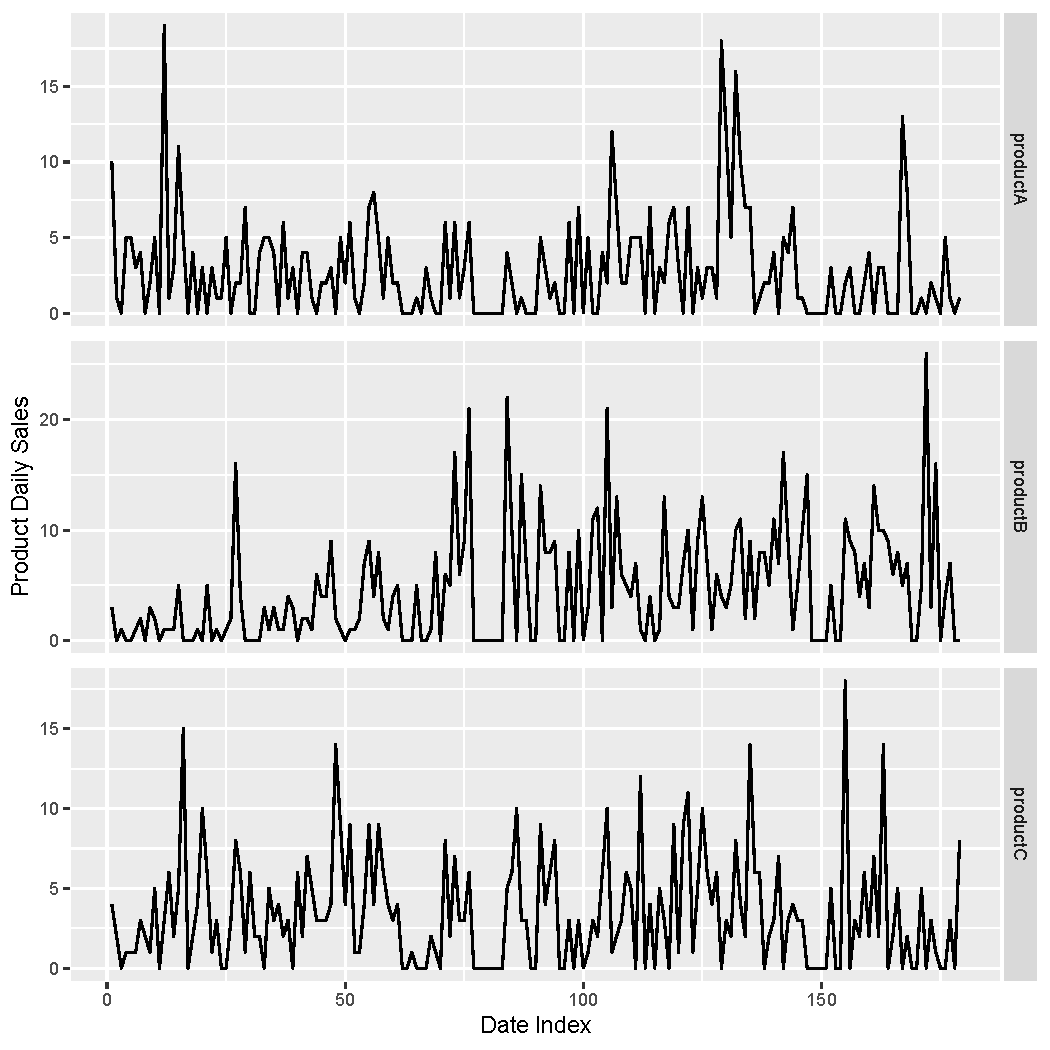
\includegraphics[scale=0.30]{images/walmart}
   \caption{\tiny {Daily sales demand of three different products over a four months period, extracted from \textit{Walmart.com} \cite{Bandara2019-bg}.}}
  \end{figure}
\end{frame}
  
\begin{frame}{Vastness of related time series}
\begin{itemize}
\item Large quantities of related, similar time series are available.
\vspace{2mm}
\begin{itemize}\color{blue}
\item The sales demand in retail of thousands of different products.
\item The emergency medical services demand in multiple local government areas.
\item The multiple server performance measures in computer centers.
\end{itemize}
\end{itemize}
\begin{itemize}
\item State-of-the-art traditional forecasting techniques are mostly univariate methods.
\vspace{2mm}
\begin{itemize}\color{blue}
\item Treat each time series separately and forecast them in isolation.
\item ETS, BaggedETS, Theta, ARIMA.
\item Unable to incorporate any key patterns and structures that may be shared by a group of time series
\item Single series may be too short to be forecast at all.
\end{itemize}
\end{itemize}

\end{frame}

\section{ML for forecasting}
  	\AtBeginSection[]
    {
      \ifnum \value{framenumber}>1
        \begin{frame}<*>
        \frametitle{Outline}
        \begin{minipage}[t]{0.48\textwidth} 
		\end{minipage}
		\begin{minipage}[t][0.6\textheight]{0.50\textwidth}
		 \vspace{0pt} 
 		 \tableofcontents[currentsection]
		\end{minipage}
        
        \end{frame}
      \else
      \fi
    } 

%\begin{frame}{Neural networks for forecasting}
		%\begin{itemize}
		%	\item Advocated as a strong alternative to traditional statistical forecasting methods.
		%	\vspace{2mm}
		%	\item Powerful computational data model.
			%\vspace{2mm}
			%\item Naturally suited to model the underlying complex relationships in data.
				%\begin{itemize}\color{blue}
				%	\item Model generalizability
				%	\item Universal function approximation properties \cite{Cybenko1989-fw,Hornik1991-wd}.
			%	\end{itemize}
			%\end{itemize}
%\end{frame}    
    
    
     
	\begin{frame}{Substandard performance in forecasting competitions}
	\begin{itemize}
	\item Sophisticated methods do not necessarily produce better forecasts than simpler ones {\cite{Makridakis2000-ih}}.
	\vspace{1.5mm}
	\begin{itemize}\color{blue}
	\item AutomatANN method in the M3 Competition.
	\end{itemize}	
	\vspace{2.0mm}
	\item Did not perform well in the subsequent competitions.
	\vspace{1.5mm}
	\begin{itemize}\color{blue}
	\item NN3 and NN5 \cite{Crone2011-vv,Crone2008-ye}.
	\item Held specifically for Computational Intelligent(CI) methods.
	\end{itemize}
	\vspace{2.0mm}
	\item Couldn't outperform simple standard methods in time series forecasting.
	\vspace{1.5mm}
	\begin{itemize}\color{blue}
	\item Theta method, simple exponential smoothing with drift \cite{Hyndman2003-kc}.
	\end{itemize}
	\end{itemize}
	\end{frame}
%   
   
   \begin{frame}{Reasons for the under-performance}
  	\begin{itemize}
  	\item Individual series are too short to be modelled effectively.
  		\vspace{1.5mm}
		\begin{itemize}\color{blue}
		\item Amount of information that can be extracted is limited.
		\item Higher probability of model over-fitting.
		\end{itemize}	
		\vspace{2.0mm}
	\item Distant past is usually not very useful for forecasting.
	\vspace{2.0mm}
	\item Neural networks do not perform well.
	  \begin{itemize}\color{blue}
		%\begin{itemize}\color{blue}
		\item Not having enough data for learning \cite{Zhang1998-tq}.
		\item Not handle non-stationarity in the data adequately \cite{Hyndman2016-ej}.
		\item Large number of hyper-parameters to be determined \cite{Yan2012-dh}.		
	  \end{itemize}		
 	\end{itemize}
   \end{frame}
%   
    \begin{frame}{Improving NNs for forecasting}
  	\begin{itemize}
	\item Preprocessing techniques.
	\vspace{0.8mm}
	  \begin{itemize}\color{blue}
		%\begin{itemize}\color{blue}
		\item Supplements the NN's learning process.
		\item deseasonalizing and detrending data prior to modelling \cite{Nelson1999-bd, Ben_Taieb2011-iu,Zhang2005-pk}.
	  \end{itemize}	
	  \vspace{1.0mm}
	\item Adapting NN architectures for forecasting
	\vspace{0.8mm}
	  \begin{itemize}\color{blue}
		%\begin{itemize}\color{blue}
		\item Ensemble architectures \cite{Rahman2016-os, Barrow2016-yv}.
		\item Generalized regression neural networks (GRNNs) \cite{Yan2012-dh}.
		\item Echo-state networks \cite{Ilies2007-ej}.
		\item Recurrent Neural Networks (RNNs) \cite{Zimmermann2012-cp,Fei2015-vh}. 
	  \end{itemize}			
 	\end{itemize}
   \end{frame}
   
   \begin{frame}{Global Forecast Models (GFMs)}
  	\begin{itemize}
  	\item Methods that estimate model parameters jointly from all available time series \cite{Januschowski2020-ud}.
	\vspace{2.0mm}
	\item A unified forecasting model that is built using all a collection of time series.
	\vspace{1.0mm}
	  \begin{itemize}\color{blue}
		%\begin{itemize}\color{blue}
		\item Borrow similar behaviours and structures from other related time series.
		\item Improves model generalizability.
		\item Adequate data for model fitting.
		\item Ability to exploit the cross-series information.
	  \end{itemize}	   
	\vspace{2.0mm}	  
	  \item Forecasting a large quantities of related time series: ``Related'' in terms of similarity of their DGP (not necessarily mere correlations)~\cite{Bergmeir2020-nu}
 	\end{itemize}
   \end{frame} 
   
  
   \begin{frame}{Scalability of GFMs}
  	\begin{itemize}
  	\item Enough data, due to more series, thus ML can be more competitive~\cite{Bergmeir2020-nu}
	\vspace{2.0mm}
	  \begin{itemize}\color{blue}
		%\begin{itemize}\color{blue}
		\item Local model: typically fitting a model with few ($<$10) parameters to a single series.
		\item If you have 10k series and fit 5 parameters, you end up with 50k parameters.
		\item Fit a global model with 5k parameters instead.
	  \end{itemize}	   
	\vspace{2.0mm}	  
	  \item Overall complexity of set of local models grows when dataset grows; complexity of global model stays the same.
 	\end{itemize}
   \end{frame}   
   
 \begin{frame}{Complexity of GFMs}
  	\begin{itemize}
  	\item  Global models can afford to be more complex.
  	\vspace{2.0mm}	  
  	\item Complexity can be added as:
  	\begin{itemize}\color{blue}
		\item Longer memory (longer input windows, more lags)
		\item Non-linear/non-parametric models (NN variants, GBT, …)
		\item Data partitioning (Time series clustering)
	  \end{itemize}
	  \vspace{2.0mm}
	  \item GFMs can be designed with a much higher complexity, yet still achieve better generalisation error than the univariate models for larger datasets \cite{Montero-Manso2021-es}
 	\end{itemize}
   \end{frame}  
   
 \begin{frame}{GFMs are not multivariate models}
  	\begin{itemize}
  	\item  Global models learn across series but predict every series in isolation.
	  \vspace{2.0mm}
	  \item They can work on datasets where series have different lengths and/or are not aligned, like the M3, M4 datasets.
	   \vspace{2.0mm}
	\item They do not take into account interactions between series.
 	\end{itemize}
   \end{frame}   
   
 \begin{frame}{Evolution of GFMs}
  	\begin{figure}
   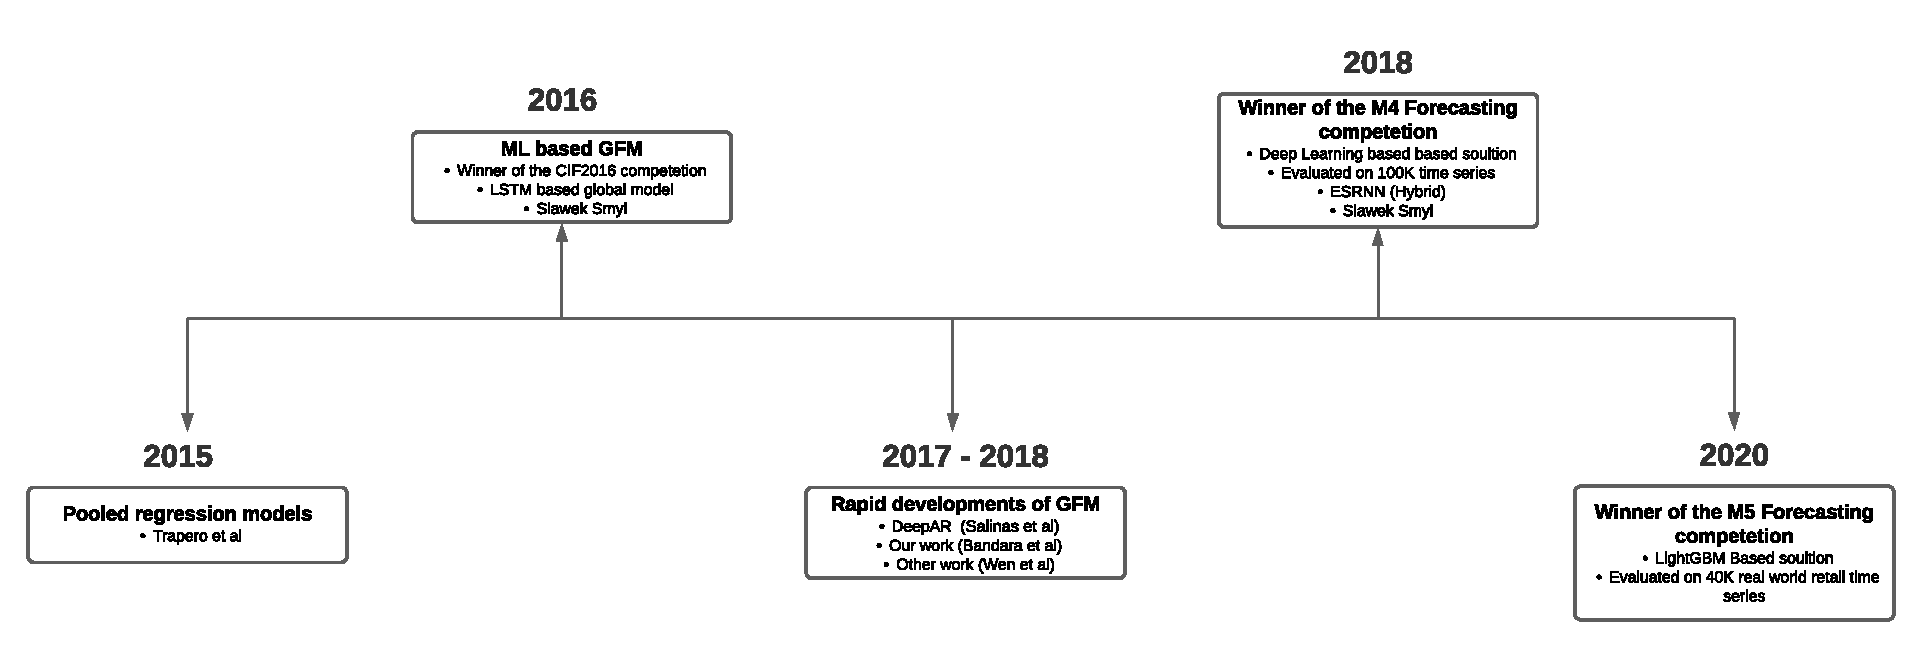
\includegraphics[scale=0.35]{images/timeline}
   \caption{\tiny{A brief overview of GFM developments}}
  \end{figure}
  \end{frame}
  
  \begin{frame}{Moving window approach}
  	 \begin{figure}[htb]
  \begin{center}
    \includegraphics[width=0.7\textwidth]{images/window_final}
    \caption{\scriptsize Applying the moving window approach over a time series . This is also known as the Multi-Input Multi-Output strategy (MIMO)}
  \label{fig:network}
  \end{center}
\end{figure}
  \end{frame}
  

\begin{frame}{Dominance in the competitions}
   	\begin{itemize}
    			\item  CIF2016 Forecasting Competition (IEEE CIS)
  				\begin{itemize}\color{blue}
						\item LSTM based GFM solution~\cite{Smyl2016-ee}
	  			\end{itemize}
   		 	\item  Wikipedia Web Traffic Forecasting (Google, 2017)
  				\begin{itemize}\color{blue}
						\item RNN based Encoder-Decoder architecture~\cite{Suilin2018-tc}
	 			 \end{itemize}
	   		\item  M4 Competition (Makridakis, 2018)
	  			 \begin{itemize}\color{blue}
					\item ES-RNN: A hybrid architecture of RNNs and exponential smoothing~\cite{Smyl2019-cb}
	 		 	\end{itemize}
	 		\item  M5 Competition (Makridakis, 2020)
	  			 \begin{itemize}\color{blue}
					\item LightGBM basedn GFM solution ~\cite{Makridakis2021-ro}
	 		 	\end{itemize}
 	\end{itemize}
 \end{frame}
 
 \begin{frame}{Deep Learning based GFMs}
   	\begin{itemize}
    			\item  The recent NLP research (LSTM, attention, transformers) is adapted to the time series use case
  				\begin{itemize}\color{blue}
						\item most recent observations are the most important ones
						\item long-term dependencies are relatively simple and stable (only seasonalities)
				\end{itemize}
   		 	\item  Recurrent Neural Network based variants
   		 		\begin{itemize}\color{blue}
						\item Overview by~\cite{Hewamalage2021-hg}
						\item Stacking, Encoder-Decoder architectures 
						\item Have an internal state which allows them to memorize.
				\end{itemize}
			\item  Convolutional neural networks
   		 		\begin{itemize}\color{blue}
						\item Competitive as RNNs, but are a lot faster to train~\cite{Borovykh2017-le}
						\item WaveNet architecture (causal convolutions, dilations)~\cite{Sen2019-jj}
				\end{itemize}
 	\end{itemize}
\end{frame} 

 \begin{frame}{Specialised architectures}
   	\begin{itemize}
    			\item  DeepAR: Generative RNN model~\cite{Salinas2020-dz}
    			  \vspace{2.0mm}
   		 	\item  Deep state space models: Parametrizes a linear state-space model with an RNN~\cite{Rangapuram2018-zq}
   		 	  \vspace{2.0mm}
   		 	\item  NBEATS~\cite{Oreshkin2019-tq}: Decomposes series into basis functions, residual stacking
   		 		\begin{itemize}\color{blue}
						\item State-of-the-art accuracy on M4 dataset.
						\item 2nd place in M5 (as part of an ensemble)
				\end{itemize}
			\item  Transformers for forecasting~\cite{Li2019-io}
			\item  Fusion Transformers~\cite{Lim2021-il}
 	\end{itemize}
\end{frame} 


 \begin{frame}{GFMs for Forecast combination}
   	\begin{itemize}
    			\item  Ensembling works in forecasting just as well as in any other area.
    			  \vspace{2.0mm}
    			\item  Local models to capture unique behaviours, Global models to capture common patterns.
    			  \vspace{2.0mm}
   		 	\item  Ensembles of local and global models
   		 		\begin{itemize}\color{blue}
						\item Energy Demand Forecasting (IEEE CIS Competition)
						\item Weekly time series forecasting~\cite{Godahewa2020-wg}
				\end{itemize}
 	\end{itemize}
\end{frame} 


%\begin{frame}{Neural networks for forecasting}
%\begin{itemize}
%\item Powerful computational data model.
%\vspace{2mm}
%\item Naturally suited to model the underlying complex relationships in data.
%\begin{itemize}\color{blue}
%\item Model generalizability
%\item Universal function approximation properties \cite{Cybenko1989-fw,Hornik1991-wd}.
%\end{itemize}
%\vspace{2mm}
%\item Advocated as a strong alternative to traditional statistical forecasting methods.
%\end{itemize}
%
%\end{frame}

    
%   \begin{frame}{Research Methods \& Objective \& Expected Outcome}
%
%    \begin{block}{Research Methods}	
%	Explore the use of HPYP/HDP smoothing techniques to decision trees and BNCs, and then to ensembles.
%	\end{block}
%    
%   \begin{block}{Research Objectives}	
%	Build Random forest and BNCs to achieve a better probability estimates.
%	\end{block}
%    
%     \begin{block}{Expected Outcome}	
%	The probability estimation of Random forest and BNCs could be improved measured by RMSE and error rate. 
%	\end{block}
%  \end{frame}


  
%% Lierature review 
%\section{Motivation}
%  	\AtBeginSection[]
%    {
%      \ifnum \value{framenumber}>1
%        \begin{frame}<*>
%        \frametitle{Outline}
%        \begin{minipage}[t]{0.48\textwidth} 
% 		\vspace{10pt}
%		\end{minipage}
%		\begin{minipage}[t][0.6\textheight]{0.50\textwidth}
%		 \vspace{0pt} 
% 		 \tableofcontents[currentsection]
%		\end{minipage}
%        
%        \end{frame}
%      \else
%      \fi
%    }    
    
%    
%	\begin{frame}{Neural networks for forecasting}
%		\begin{itemize}
%			\item Powerful computational data model.
%			\vspace{2mm}
%			\item Naturally suited to model the underlying complex relationships in data.
%				\begin{itemize}\color{blue}
%					\item Model generalizability
%					\item Universal function approximation properties \cite{Cybenko1989-fw,Hornik1991-wd}.
%				\end{itemize}
%			\vspace{2mm}
%			\item Advocated as a strong alternative to traditional statistical forecasting methods.
%			\end{itemize}
%	\end{frame}    
%    
%    
%     
%	\begin{frame}{Substandard performance in forecasting competitions}
%	\begin{itemize}
%	\item Uncompetitive results of NN variants in the M3 forecasting competition {\cite{Makridakis2000-ih}}.
%	\vspace{1.5mm}
%	\begin{itemize}\color{blue}
%	\item Simple methods will often outperform more sophisticated ones.
%	\end{itemize}	
%	\vspace{2.0mm}
%	\item Did not perform well in the subsequent competitions.
%	\vspace{1.5mm}
%	\begin{itemize}\color{blue}
%	\item NN3 and NN5 \cite{Crone2011-vv,Crone2008-ye}.
%	\item Held specifically for Computational Intelligent(CI) methods.
%	\end{itemize}
%	\vspace{2.0mm}
%	\item Couldn't outperform simple standard methods in time series forecasting.
%	\vspace{1.5mm}
%	\begin{itemize}\color{blue}
%	\item Theta method, simple exponential smoothing with drift \cite{Hyndman2003-kc}.
%	\end{itemize}
%	\end{itemize}
%	\end{frame}
%   
%   
%   \begin{frame}{Reasons for the under-performance}
%  	\begin{itemize}
%  	\item Individual series are too short to be modelled effectively.
%  		\vspace{1.5mm}
%		\begin{itemize}\color{blue}
%		\item Amount of information that can be extracted is limited.
%		\item More complex methods $\Rightarrow$ \textbf{smaller bias}  $\Rightarrow$ \textbf{large variance}. 
%		\end{itemize}	
%		\vspace{2.0mm}
%	\item Distant past is usually not very useful for forecasting.
%	\vspace{2.0mm}
%	\item Neural networks do not perform well.
%	  \begin{itemize}\color{blue}
%		%\begin{itemize}\color{blue}
%		\item Not having enough data for learning \cite{Zhang1998-tq}.
%		\item Not handle non-stationarity in the data adequately \cite{Hyndman2016-ej}.
%		\item Large number of hyper-parameters to be determined \cite{Yan2012-dh}.		
%	  \end{itemize}		
% 	\end{itemize}
%   \end{frame}
   
   
%   \begin{frame}{Uplifting NNs for forecasting}
%  	\begin{itemize}
%  	\item Honing NN's performance on time series data.
%	\vspace{1.0mm}
%	\item Preprocessing techniques
%	\vspace{0.8mm}
%	  \begin{itemize}\color{blue}
%		%\begin{itemize}\color{blue}
%		\item Supplements the NN's learning process.
%		\item deseasonalizing and detrending data prior to modelling \cite{Nelson1999-bd, Ben_Taieb2011-iu,Zhang2005-pk}.
%	  \end{itemize}	
%	  \vspace{1.0mm}
%	\item Adapting NN architectures for forecasting
%	\vspace{0.8mm}
%	  \begin{itemize}\color{blue}
%		%\begin{itemize}\color{blue}
%		\item Ensemble architectures \cite{Rahman2016-os, Barrow2016-yv}.
%		\item Generalized regression neural networks (GRNNs) \cite{Yan2012-dh}.
%		\item Echo-state networks \cite{Ilies2007-tz}.
%		\item Recurrent Neural Networks (RNNs) \cite{Zimmermann2012-cp,Fei2015-vh}. 
%	  \end{itemize}			
% 	\end{itemize}
%   \end{frame}
   
%	 \begin{frame}{Challenges in Global Forecast Models (GFMs)}
%  	\begin{itemize}
%	  \item Encompassed with various challenges to improve the forecast accuracy.
%	  \vspace{1.8mm} 
%	  	\vspace{0.8mm}
%	  	\begin{itemize}\color{blue}	  	
%		\item Account for the disparity factor of a global models, when trained across heterogeneous set of time series.
%		\item Handle multiple seasonal patterns in a group of time series.
%		\item Improving forecast accuracy in situations where number of available time series are limited.
%		\item Empirical evidence from real-world applications.
%	  \end{itemize}
% 	\end{itemize}
%   \end{frame} 
%    \begin{frame}{Exploiting cross-series information}
%  	\begin{itemize}
%	\item Applied NN in the form of univariate time forecasting method.
%	\vspace{0.8mm}
%	  \begin{itemize}\color{blue}
%		%\begin{itemize}\color{blue}
%		\item Disregards the cross-series information available from sets of time series.
%	  \end{itemize}	
%	  \vspace{1.0mm}
%	\item  Studies examined to incorporate cross-series information.
%	\vspace{0.8mm}
%	  \begin{itemize}\color{blue}
%%		%\begin{itemize}\color{blue}
%		\item Regression model on set of related time series \cite{Hartmann2015-uu}.
%		\item LSTM approach trained across all available time series \cite{Smyl2016-ee}.
%%		\item Recurrent Neural Networks (RNNs) \cite{Zimmermann2012-cp,Fei2015-vh}
%	  \end{itemize}			
% 	\end{itemize}
%   \end{frame}    


%	\begin{frame}{Generalized regression neural networks (GRNNs)}
%  	\begin{itemize}
%	  \item Address the design implications associate with traditional NNs.
%	  	\vspace{0.8mm}
%	  \begin{itemize}\color{blue}
%%		%\begin{itemize}\color{blue}
%		\item Large number of design parameters.
%		\item Long training time.
%		\item Learning constraints (suffers from local minima).
%	  \end{itemize}
%	  \vspace{1.8mm}
%	  \item A special type of neural network (GRNN) \cite{Yan2012-dh}.
%	  	\vspace{0.8mm}
%	  	\begin{itemize}\color{blue}
%		\item Contains only single design parameter.
%		\item Relatively fast training procedure.
%		\item Fusing multiple GRNNs.
%	  \end{itemize}
% 	\end{itemize}
%   \end{frame} 
   
%     	\begin{frame}{RNN architectures for forecasting}
%  	\begin{itemize}
%	\item Capturing dependencies in span of contextual information.
%	\vspace{0.8mm}
%	  \begin{itemize}\color{blue}
%		%\begin{itemize}\color{blue}
%		\item Time series is a representation of sequence of data points ordered in a time space.
%		\vspace{0.4mm}
%		\item Naturally suited to model time series data.
%	  \end{itemize}	   
%	\vspace{1.0mm}	  
%	  \item Once again used as a univariate forecasting model.
%	  \vspace{0.8mm}
%	  \begin{itemize}\color{blue}
%		%\begin{itemize}\color{blue}
%		\item Predicting drop-out-rates of the massive open online courses \cite{Fei2015-vh}.
%		\vspace{0.4mm}
%		\item Forecasting clinical measurements of the ICU patients \cite{Lipton2015-vj}.
%		\vspace{0.4mm}
%		\item Travel time and Short-term Traffic-flow prediction \cite{Tian2015-nz,Duan2016-ta}.
%	  \end{itemize}	   
% 	\end{itemize}
%   \end{frame}   
   

%	 \begin{frame}{Exploiting cross-series information}
%  	\begin{itemize}
%	\item Many studies applied NN in the form of univariate time forecasting method.
%	\vspace{0.6mm}
%	  \begin{itemize}\color{blue}
%		%\begin{itemize}\color{blue}
%		\item Disregards the cross-series information available from sets of time series.
%	  \end{itemize}	
%	  \vspace{1.0mm}
%	\item  Studies examined to incorporate cross-series information.
%	\vspace{0.8mm}
%	  \begin{itemize}\color{blue}
%%		%\begin{itemize}\color{blue}
%		\item Regression model on set of related time series \cite{Hartmann2015-uu}.
%		\item LSTM approach trained across all available time series \cite{Smyl2016-ee}.
%%		\item Recurrent Neural Networks (RNNs) \cite{Zimmermann2012-cp,Fei2015-vh}
%	  \end{itemize}			
% 	\end{itemize}
%   \end{frame}   
   
	
%	 \begin{frame}{Recent Success \normalsize{\cite{Smyl2016-ee}}}
%  	\begin{itemize}
%	\item LSTM approach trained across all available time series.
%	\vspace{0.8mm}
%	  \begin{itemize}\color{blue}
%		%\begin{itemize}\color{blue}
%		\item Special type of Recurrent neural network (RNN).
%		\item Accounts for information dispersed across many similar series.
%		\item One forecasting model across whole set of time series.
%		\item Winner of the CIF2016 forecasting competition.
%		\item Outperforms all state-of-the-art univariate algorithms.
%		%\item Winner of the CIF 2016 forecasting competition.
%	  \end{itemize}	
%	  \vspace{2.0mm}
%	\item CIF2016 competition \cite{Stepnicka2016-bu}.
%	\vspace{0.8mm}
%	  \begin{itemize}\color{blue}
%%%		%\begin{itemize}\color{blue}
%		\item Monthly time series.
%		\item Comprised of similar time series related to the banking industry.
%%		\item LSTM approach trained across all available time series \cite{Smyl2016-ee}.
%%%		\item Recurrent Neural Networks (RNNs) \cite{Zimmermann2012-cp,Fei2015-vh}
%	  \end{itemize}			
% 	\end{itemize}
%   \end{frame}  
   
%   	\begin{frame}{Forecasting across similar time series databases}
%  	\begin{itemize}
%  	\item Large quantities of similar time series are available (Big-Data, in the time series context). 
%	\vspace{2.0mm}
%	\item Building global models on similar set of time series.
%	\vspace{2.0mm}
%	\item Presence of heterogeneous set of time series.
%	\vspace{1.0mm}
%	  \begin{itemize}\color{blue}
%		%\begin{itemize}\color{blue}
%		\item Learning across disparate sets of time series.
%		\item Accuracy of these models can be degenerated.
%	  \end{itemize}	   
%	\vspace{2.0mm}	  
%	  \item A notion of similarity between the time series needs to be built into the methods.
% 	\end{itemize}
%   \end{frame}   
   
%	 \begin{frame}{Research Objectives}
%  		 \begin{block}{Research Objective 1: (RO1)}
%  		 A notion of similarity between the time series needs to be built into the global methods to identify and account for the time series with homogeneous characteristics.
%	\end{block} 
%		\begin{block}{Research Objective 2: (RO2)}	
%		 Time series may exhibit complex seasonal patterns such as multiple seasonal
%patterns, non-integer seasonality, calender effects. We extend the developments in \textbf{(RO1)} to accommodate time series with multiple seasonal cycles.
%	\end{block}
%  \end{frame}  
%  
%   \begin{frame}{Research Objectives Cont.}
%  		 \begin{block}{Research Objective 3: (RO3)}
%  		The unified forecasting models are often constrained by the amount of time
%series available in a database. To this end, we use augmentation techniques to synthetically increase the number of available time series.
%	\end{block} 
%		\begin{block}{Research Objective 4: (RO4)}	
%		 The outcomes of \textbf{RO1, RO2 and RO3}, will position us to apply
%our developments to address the real-world challenges in the industry. More specifically, we aim to apply our developments to predict the future demand of the emergency services in the health-care domain.
%	\end{block}
%  \end{frame}  
     
%   
  


%\begin{frame}{Research Questions}
%  		 \begin{block}{Research Question 1: (RQ1)}
%  		Does building a notion of similarity between the time series assist the GFMs
%to distinguish the variations exist among a group of time series ?
%	\end{block} 
%		\begin{block}{Research Question 2: (RQ2)}	
%		How various forms of multi-seasonal decomposition techniques can supplement the learning process of GFMs, when forecasting a group of time series with multiple seasonal cycles ?
%	\end{block}
%  \end{frame} 
% \begin{frame}{Research Questions Cont.}
%	\begin{block}{Research Question 3: (RQ3)}	
%		Can we successfully leverage the development versions of  \textbf{RQ1, RQ2} to address the various forecasting challenges that exist in the Emergency Medical Services domain ?
%	\end{block}
%	\begin{block}{Research Question 4: (RQ4)}	
%		Can transfer learning approaches uplift the forecast accuracy of GFMs, in
%situations where the availability of time series is limited ?
%	\end{block}
%  \end{frame} 
  
  
%\begin{frame}{Research Contributions}
%	\begin{itemize}
%		\item A forecasting framework that exploits the cross-series information in a set of time series by building separate models for subgroups of time series, specified
%by a time series clustering methodology (\textbf{RQ1}).
%		\item A forecasting framework to exploit sales demand relationships available in an E-commerce product hierarchy, and an empirical evaluation of the proposed framework using a real-world retail sales dataset.
%(\textbf{RQ1})
%	\item A decomposition based, unified prediction framework to forecast time series with multiple seasonal patterns (\textbf{RQ2}).
%	\end{itemize}	
%\end{frame}
%
%\begin{frame}{Research Contributions Cont.}
%\begin{itemize}
%		\item Developing a global forecasting and inference framework to forecast the Emergency Medical Services (EMS) demand, analyse causal relationships, and perform `what-if' analyses for policy-making across multiple local government areas (\textbf{RQ3}).
%		\vspace{2mm}
%		\item Developing transfer learning schemes for GFMs to uplift the forecast accuracy in situations with limited number of time series (\textbf{RQ4}).
%\end{itemize}
%\end{frame}

%\section{Recurrent Neural Networks}

 	%\AtBeginSection[]
  %  {
    %  \ifnum \value{framenumber}>1
     %   \begin{frame}<*>
      %  \frametitle{Outline}
      %  \begin{minipage}[t]{0.48\textwidth}
		%\end{minipage}
		%\begin{minipage}[t][0.6\textheight]{0.50\textwidth}
		% \vspace{0pt} 
 		% \tableofcontents[currentsection]
		%\end{minipage}
       % \end{frame}
     % \else
    %  \fi
%   % }       
%
%\begin{frame}{Recurrent Neural Networks \normalsize{\cite{Elman1990-my}}}
%	\begin{figure}
%   \includegraphics[scale=0.14]{rnn_3}
%   \caption{\scriptsize {An unrolled recurrent neural network in time, with the shared weights of $U$, $V$, and $W$. The matrices $U$ $\in$ ${\Bbb R^{m \times n}}$, $W$ $\in$ ${\Bbb R^{n \times n}}$, and $V$ $\in$ ${\Bbb R^{n \times k}}$ define the shared weights of the RNN. Here, $n$, $m$, and $k$ represent the sizes of state, input, and output vectors.}}
%  \end{figure} 	
%   \end{frame}  
   
%\begin{frame}{Recurrent Neural Networks}
%\begin{align*}
%  h_t             & = f_{\theta}(Ux_t + Wh_{t-1})\\
%  o_t             & = softmax(Vh_t)
%\end{align*}

%  	\begin{itemize}
%	\item In addition to the standard input and output layer, RNNs contain special
%hidden layers that are composed of recurrently connected nodes.
%	\vspace{0.8mm}
%	  \begin{itemize}\color{blue}
%		\item Hidden layers are commonly referred to as memory states.
%		\item Enables the network to preserve the sequential information and persist the knowledge acquired from subsequent time steps.
%		\item Speech recognition, Language modelling and translation.
%	  \end{itemize}		
% 	\end{itemize}
%   \end{frame}
   
   
%\begin{frame}{RNNs vs ARIMA}
%\begin{itemize}
%	\item General class of an ARMA(p,q):
%\end{itemize}
%\begin{align*}
%     x_{t} =  c+ \sum_{i=1}^{p}\phi_{i}x_{t-i} + \sum_{j=1}^{q}\theta_{j}\varepsilon_{t-j} + \varepsilon_{t}           
%\end{align*}
%\begin{itemize}
%	\item Non-linear generalization of the linear ARMA: NARMA(p,q)
%		\begin{itemize}\color{blue}
%		\item Non-linear autoregressive models: Time lagged observations.
%		\item Weighted moving average terms: BPTT algorithm.
%	  \end{itemize}	
%\end{itemize}
%\begin{align*}
%     y_{t} =   g(y_{t-1},y_{t-2},\cdots, y_{t-p},\varepsilon_{t-1}, \varepsilon_{t-2}, \cdots ,\varepsilon_{t-q}) + \varepsilon_{t}
%\end{align*}
%\end{frame} 


%\begin{frame}{Highlights of RNN}
%\begin{itemize}
%	\item Capable of capturing short-term dependencies in sequential data.
%	\item Difficulties in learning long-term dependencies from distant
%past information.
%	\item Caused by the \textit{vanishing gradient problem}.
%	\item Well-known constraint in gradient based learning algorithms.
%	\item Novel RNN architectures, such as LSTM (Long Short-Term Memory Networks), GRU (Gated Recurrent Units) introduced.
%\end{itemize}
%\end{frame} 

%\begin{frame}{Moving window approach}
%   \begin{figure}[htb]
%  \begin{center}
%    \includegraphics[width=0.7\textwidth]{window_final}
%    \caption{\scriptsize Applying the moving window approach over a time series . This is also known as the Multi-Input Multi-Output strategy (MIMO)}
%  \label{fig:network}
%  \end{center}
%\end{figure}
% \end{frame}     
   

 
\section{Research Projects}

 	\AtBeginSection[]
    {
      \ifnum \value{framenumber}>1
        \begin{frame}<*>
        \frametitle{Outline}
        \begin{minipage}[t]{0.48\textwidth} 
 		\vspace{10pt}
		\end{minipage}
		\begin{minipage}[t][0.6\textheight]{0.50\textwidth}
		 \vspace{0pt} 
 		 \tableofcontents[currentsection]
		\end{minipage}
        
        \end{frame}
      \else
      \fi
    }
    
\begin{frame}{Research Project 1}
   \begin{block}{Research Question}	
	Does building a notion of similarity between the time series assist the GFMs to distinguish the variations exist among a group of time series.
	\end{block}
	\vspace{0.8mm}
	\begin{itemize}
	\item Learning across these disparate set of time series may degenerate the overall accuracy of GFM models.
	\item A notion of similarity between the time series needs to be built into the global methods.
	\item Identify and account for the time series with homogeneous characteristics.
	\end{itemize}
\end{frame}  


\begin{frame}{Research Project 1: Approach}
	\begin{itemize}
	\item Building GFMs on subgroups of similar time series.
	\begin{itemize}\color{blue}
		\item The Long Short-Term Memory Neural Networks (LSTMs) used as the primary GFM.
		\item The similarity is captured through clustering the time series into subgroups.
		\item Feature based clustering approach using kMeans, DBScan, Partition Around Medoids (PAM),
and Snob.
	\end{itemize}
	\vspace{0.8mm}
	\item A prior time series clustering can supplement the GFM training procedure by improving the homogeneousness of the trainable time series.
	\begin{itemize}\color{blue}
		\item Achieves competitive results on benchmarking datasets under competition evaluation procedures.
	\end{itemize}
\end{itemize}
\end{frame} 

\begin{frame}{Research Project 1: Overall Architecture}
 \begin{figure}[htb]
  \begin{center}
    
\includegraphics[width=0.4\textwidth]{images/architecture_final2}
    \caption{Pre-processing layer, LSTM training layer and a Post-processing layer.}
  \label{fig:network}
  \end{center}
\end{figure}
\end{frame} 


\begin{frame}{Research Project 2}
	\begin{itemize}
	\item Applying the clustering based GFM framework to forecast the demand in a E-commerce product assortment hierarchy
	\begin{itemize}\color{blue}
		\item A product grouping strategy introduced to supplement the GFM learning schemes, in situations where sales patterns in a product portfolio are disparate.
	\end{itemize}
	\vspace{0.8mm}
	\item Empirically evaluated using real-world retail sales data from Walmart.com
	\begin{itemize}\color{blue}
		\item A combination of static and dynamic features to model time series characteristics.
		\item Product class, Product category, Calendar information (holidays, season etc.)
		\item Evaluated on 20,000 items in the portfolio. 
		\item Outperforms the current forecasting pipeline at Walmart and many standard benchmarks.
	\end{itemize}
	\end{itemize}
\end{frame}

\begin{frame}{Research Project 2: Overall Architecture}
\begin{figure}[htbp]

\centerline{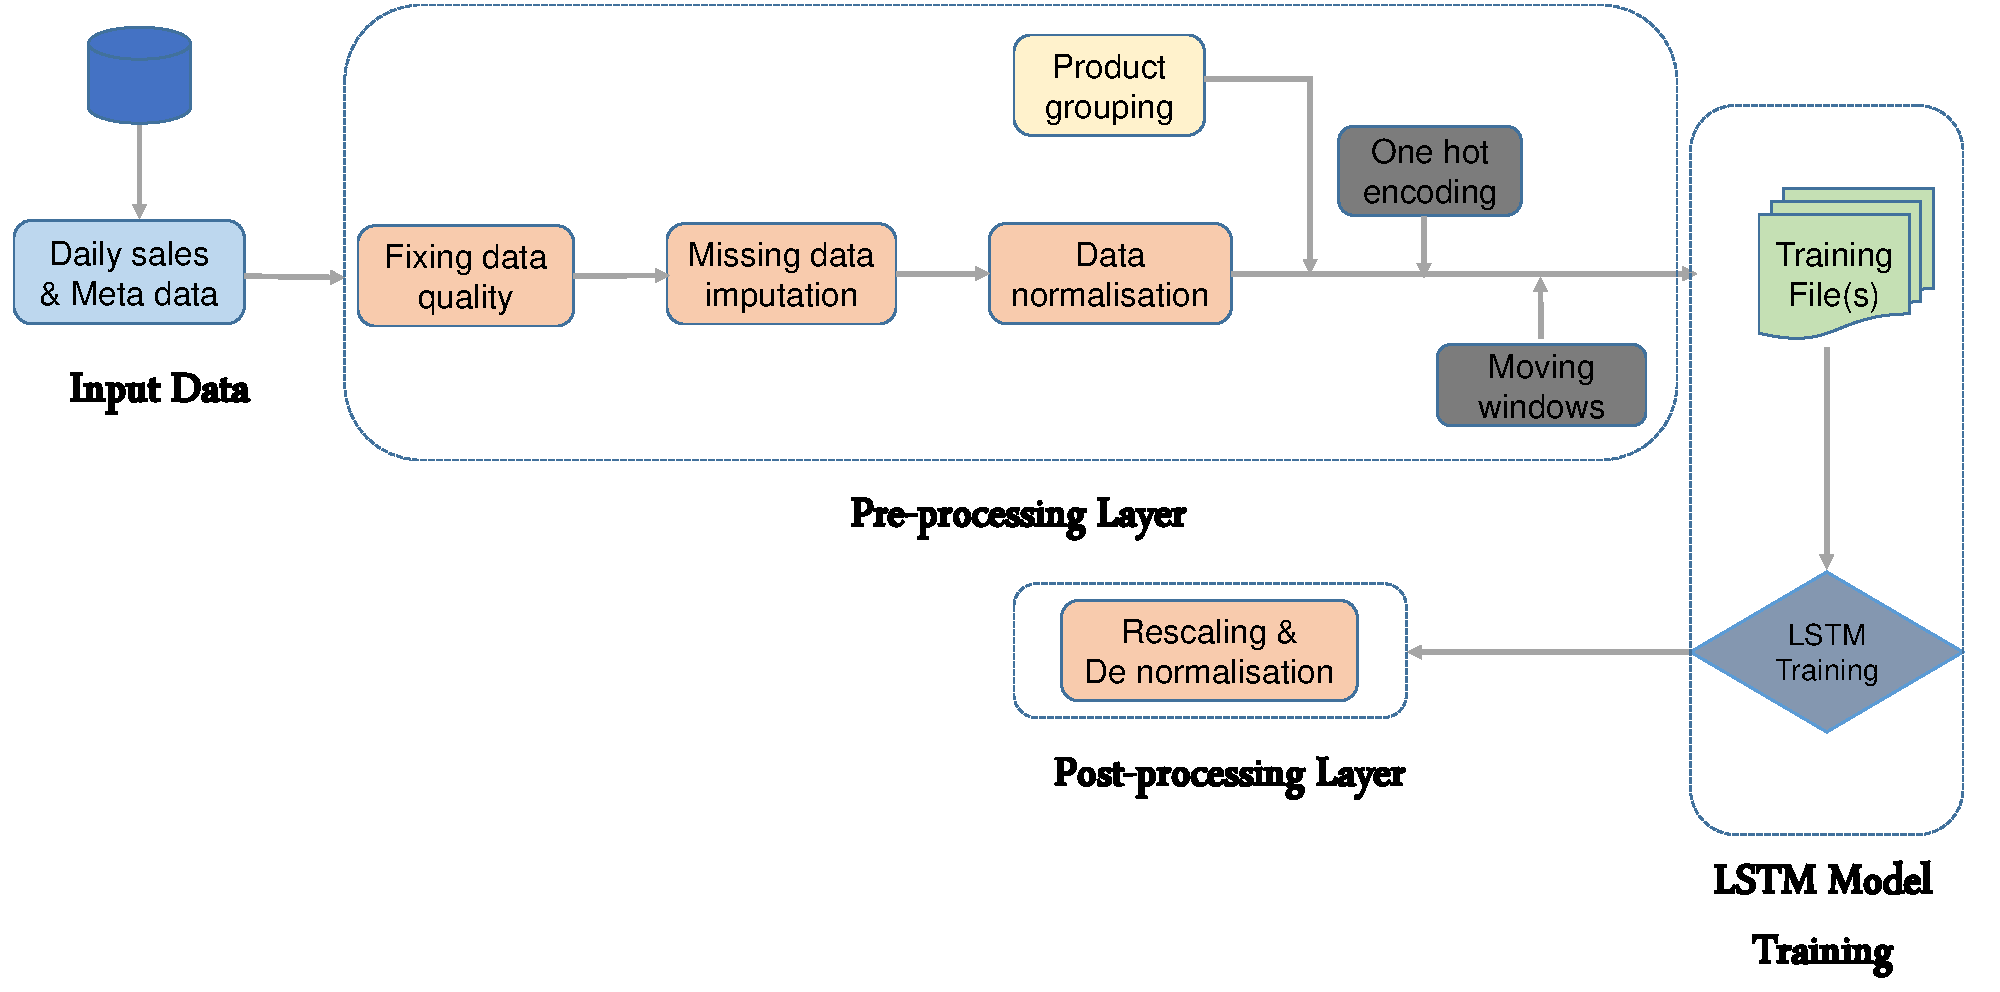
\includegraphics[width=1.10\textwidth]{images/system_diagram}}

\caption{ \scriptsize An overview of the proposed sales demand forecasting framework, which consists of a pre-processing, an LSTM training, and a post-processing part}

\label{process}

\end{figure}
\end{frame}


%\begin{frame}{Publications and Presentations}
%	\small
%\begin{enumerate}
%    \item \textcolor{blue}{Forecasting sets of similar time series with recurrent neural networks}\\
%    Authors: Kasun Bandara, Christoph Bergmeir, Slawek Smyl \\
%    Abstract accepted at the \textit{International Symposium on Forecasting (ISF) 2017}.
%    \vspace{3mm}
%    \item \textcolor{blue}{Forecasting Across Time Series Databases using Recurrent Neural Networks on Groups of Similar Series: A Clustering Approach}\\
%    Authors: Kasun Bandara, Christoph Bergmeir, Slawek Smyl \\
%    Journal acceptance at \textit{Expert Systems With Applications}.
%\end{enumerate}
%\end{frame}

%\begin{frame}{Publications and Presentations Cont.}
%	\small
%\begin{enumerate}
%\setcounter{enumi}{3}
%	 \item \textcolor{blue}{Sales Demand Forecast in E-commerce using a Long Short-Term Memory Neural Network Methodology}\\
%    Authors: Kasun Bandara, Peibei Shi, Christoph Bergmeir, Hansika Hewamalage, Quoc Tran, Brian Seaman \\
%    Conference acceptance at \textit{International Conference on Neural Information Processing (ICONIP 2019)}.
%     \vspace{3mm}
%    \item \textcolor{blue}{Industry Presentations}\\
%    Presentations on my research work to leading retailers in Australia (Coles, Bunnings), and discuss in which they can incorporate to improve their forecasting pipeline.\\
%\end{enumerate}
%\end{frame}

\begin{frame}{Research Project 3}
   \begin{block}{Research Question}	
	How various forms of multi-seasonal decomposition techniques can supplement the learning process of GFMs, when forecasting a group of time series with multiple seasonal cycles.
	\end{block}
	\begin{itemize}
	\item Time series may exhibit complex behaviours.
		\begin{itemize}
		\item \color{blue} Non-integer seasonality, Calendar effects, \textbf{Multiple seasonal patterns}.
		\end{itemize}
	\item Time series with higher sampling rates (sub-hourly, hourly, daily) are becoming more common in many industries.
		\begin{itemize}
\item \color{blue} Utility demand industry (electricity and water usage).
\item \color{blue} Transportation, Tourist, and Health care industries.
		\end{itemize}
%\item Accurate modelling of multiple seasonal cycles is necessary to estimate the demand on various time horizons precisely.
 \end{itemize}
\end{frame} 

\begin{frame}{Research Project 3: Approach}
\begin{itemize}
	\item A decomposition based, GFM based prediction framework to forecast time series with multiple seasonal patterns.
	\vspace{3mm}
	\item Using state-of-the-art multiseasonal decomposition techniques to supplement the RNN based GFM learning procedure.
	\vspace{2mm}
	  \begin{itemize}\color{blue}
		\item Seasonal decomposition is advocated by many studies \cite{Ben_Taieb2011-iu,Zhang2005-pk}.
		\item Supplements the RNN's learning process.
		\item Deseasonalized Approach: Seasonally adjusted time series
		\item Seasonal Exogenous Approach: Seasonal components as external regressors.
	  \end{itemize}			
 	\end{itemize}
\end{frame}


\begin{frame}{Research Project 3: Overall Architecture}
  	\begin{figure}[htp]
\subfloat[The proposed DS training paradigm used to train the LSTM-MSNet]{%
  \centerline{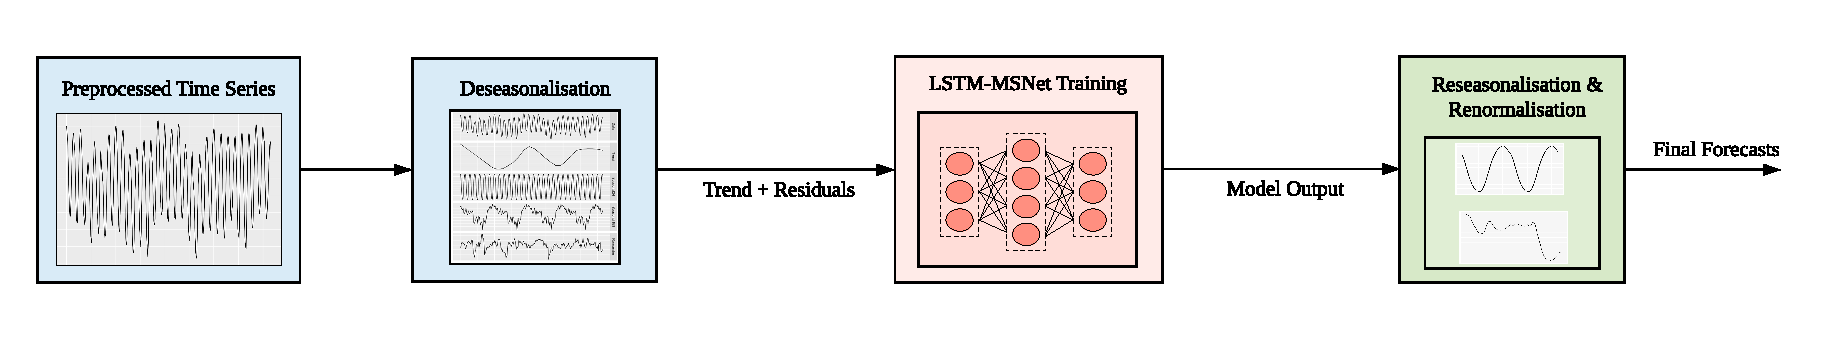
\includegraphics[width=0.80\textwidth]{images/lstm1}}
}
\vspace{4mm}
\subfloat[The proposed SE training paradigm used to train the LSTM-MSNet]{%
  \centerline{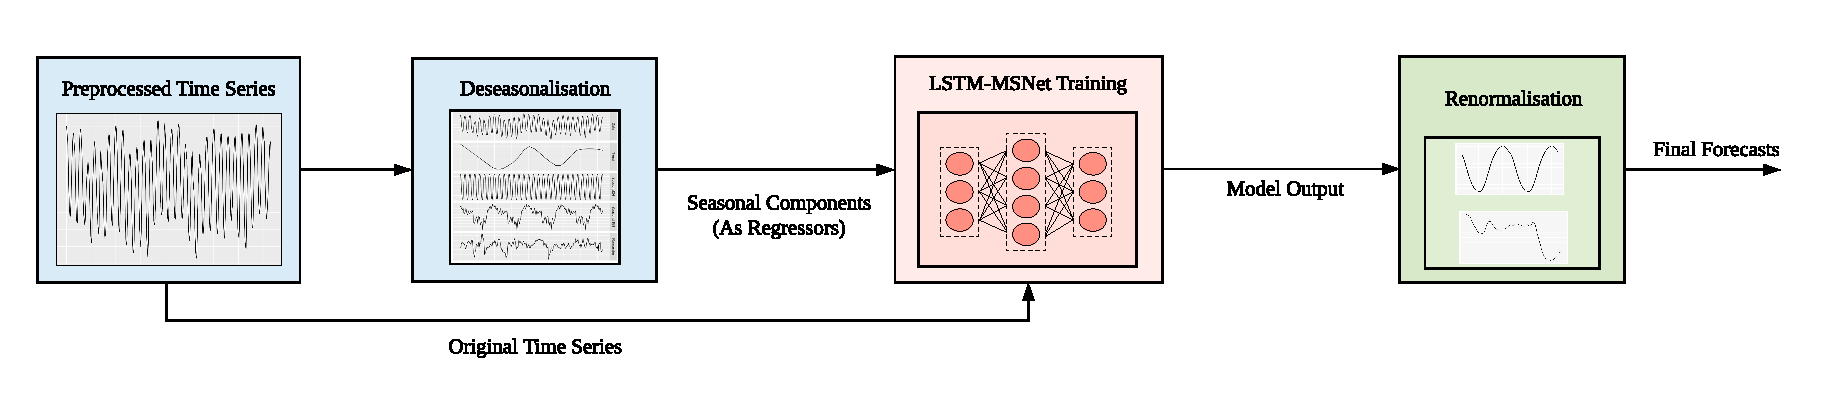
\includegraphics[width=0.80\textwidth]{images/lstm2}}
}
\caption{\tiny An overview of the proposed LSTM-MSNet training paradigms. In the DS approach, deseasonalised time series are used to train the LSTM-MSNet. Whereas in the SE approach, the seasonal values extracted from the deseasonalisation phase are employed as exogenous variables, along with the original time series to train the LSTM-MSNet.}
\label{lstm-schemes}
\end{figure}

\end{frame}

\begin{frame}{Research Project 3: Major Findings}
  	\begin{figure}[htbp]
\centerline{\includegraphics[width=0.32\textwidth]{images/seasonality_pattern}}
\caption{\tiny The seasonal components' distributions of the sum of multiple seasonalities extracted from the AusGrid-Energy (half hourly), AusGrid-Energy (hourly), M4 and the Traffic datasets, by applying the MSTL decomposition technique to the initial 200 data points of each time series.}
\label{seasonalpatterns}
\end{figure}
\end{frame}
%
%\begin{frame}{Research Project 3: Publications and Achievements}
%	\small
%\begin{enumerate}
%    \item \textcolor{blue}{Forecasting Time Series with Multiple Seasonal Patterns using a Long Short-Term Memory Neural Network Methodology}\\
%    Authors: Kasun Bandara, Christoph Bergmeir, Hansika Hewamalage \\
%    Abstract accepted at the \textit{International Symposium on Forecasting (ISF 2019)}.
%    \vspace{3mm}
%    \item \textcolor{blue}{LSTM-MSNet: Leveraging Forecasts on Sets of Related Time Series with Multiple Seasonal Patterns}\\
%    Authors: Kasun Bandara, Christoph Bergmeir, Hansika Hewamalage \\
%    Accepted for publication in \textit{IEEE Transactions on Neural Networks and Learning Systems}.
%\end{enumerate}
%\end{frame}

%\begin{frame}{Research Project 4}
%   \begin{block}{Research Question}	
%	Can we successfully leverage the previous developments to address the various forecasting challenges that exist in the Emergency Medical Services domain.
%	\end{block}
%	\begin{itemize}
%	\item Predicting future demand of the Emergency Medical Services (EMS) is a critical task.
%		\begin{itemize}
%		\item \color{blue} Efficient resource management strategy to allocate the available medical resources, i.e., number of paramedics and size of ambulances fleets.
%			\item \color{blue} Deliver high-quality medical services for the urgent patients in a timely manner.
%		\end{itemize}
% \end{itemize}
%\end{frame}


\begin{frame}{Research Project 4: DeepPPMNet}
	\begin{itemize}
	\item GFM allows to train across all the available EMS demand time series to exploit the potential cross-series information available in multiple local governing areas (LGAs).
	\vspace{4mm}
	\item Capable of exploring the causal relationships using the notion of Granger Causality, where the GFM enables to perform ‘what-if’ analyses.
	\begin{itemize}\color{blue}
		\item Using potential external regressors to evaluate whether the
base accuracies are improved.
		\item Sensitivity analysis to assess their impact towards EMS.
		\item GFMs make the ‘what-if’ analysis feasible even for relatively
constant features.
		\item Allows government decision makers to assess the factors that
could drive the EMS demand.
	\end{itemize}
\end{itemize}
\end{frame} 

\begin{frame}{Research Project 4: Evaluation}
	\begin{itemize}
	\item The DeepPPMNet was evaluated using a realworld EMS demand dataset
	\vspace{1mm}
	\begin{itemize}\color{blue}
		\item National dataset of coded ambulance clinical records held by Turning Point, an Australian addiction research and education centre.
		\item Related to alcohol overdose, suicide attempts, and other drug related harms.
		\item 8 years worth of EMS related data for each LGA.
		\item Our methods outperform state-of-the-art univariate time series models.
	\end{itemize}
	\item A case study to investiage the use of DeepPPMNet
	\vspace{2mm}
	\begin{itemize}\color{blue}
		\item How the number of alcohol licenses issued (ALI) for a certain period of time can affect the alcohol related EMS demand patterns.
	\end{itemize}
\end{itemize}
\end{frame}

\begin{frame}{Research Project 4: DeepPPMNet Case Study}
\begin{figure}[htbp]
\centerline{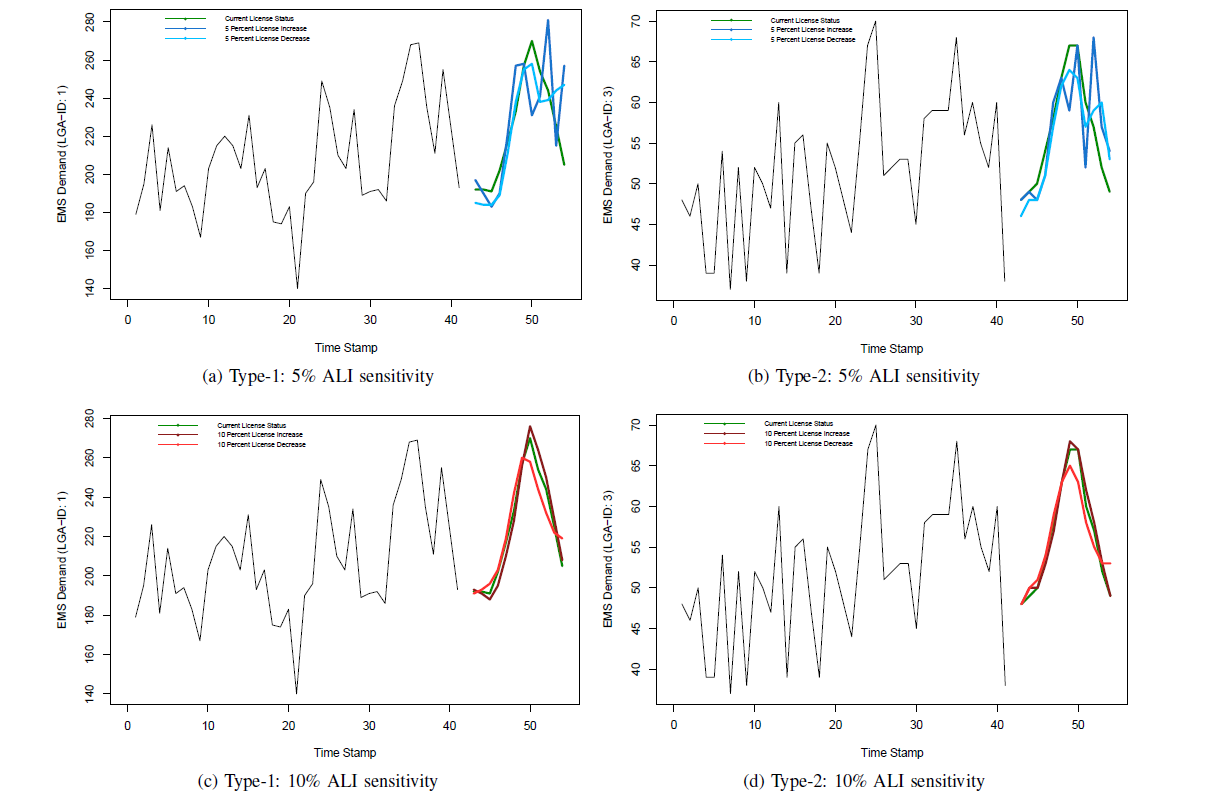
\includegraphics[width=0.80\textwidth]{images/whatif}}
\caption{ \scriptsize The application of `what-if' scenario analysis, using the number of  ALI (as a percentage of change) against the AO related EMS demand.}
\label{whatif}
\end{figure}
\end{frame}

\begin{frame}{Research Project 5 }
   \begin{block}{Research Question}	
	The effectiveness of using global models for causal Inference through Counterfactual Prediction
	\end{block}
	\begin{itemize}
	\item Global model based Recurrent neural networks (RNN) to predict policy interventions’ causal effects on an outcome over time through the counterfactual approach.
		\begin{itemize}
		\item \color{blue} Traditional methods hold strong linearity and convexity assumptions in covariates, leading us to an non realistic fitting
		\item \color{blue}  Synthetic Control Method, Google Causal Impact
		\item \color{blue} Limitations of equivalence assumption between the control and treated units distribution in the pre-treatment period.
		\end{itemize}
 \end{itemize}
\end{frame}

\begin{frame}{Causal inference}
\begin{figure}[htbp]
\centerline{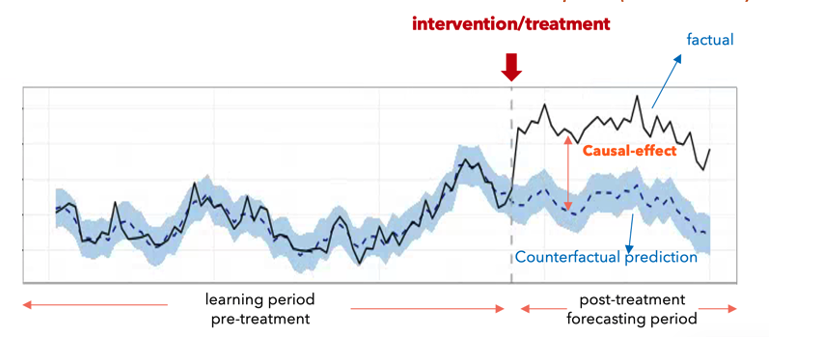
\includegraphics[width=0.90\textwidth]{images/causal}}
\caption{ \scriptsize Generating counterfactual predictions for the units affected by intervention (treated units) based on a large-dimensional panel of observed time-series from a pool of untreated peers (control units)}
\label{causal}
\end{figure}
\end{frame}


\begin{frame}{Generating counterfactuals from DeepCPNet}
	\begin{itemize}
	\item GFM is trained across all the panel of treated and control times series, before the intervention.
	\vspace{2mm}
	\item Predicts the counterfactual trajectory for the treated unit simulating its behaviour in the absence of the intervention, after the intervention.
	\vspace{2mm}
	\item Placebo tests to evaluate the counterfactual predictions
	\begin{itemize}\color{blue}
		\item Null Effect of the treatment for the control units: performance of the model only over the forecasting of the control group.
		\item The significance of the differences between the effects: the difference between the errors from treated and control units must be statistically significant (non-parametric paired Wilcoxon signed-rank)
	\end{itemize}
\end{itemize}
\end{frame} 


\begin{frame}{Effect of COVID19 lockdown measures}
\begin{figure}[htbp]
\centerline{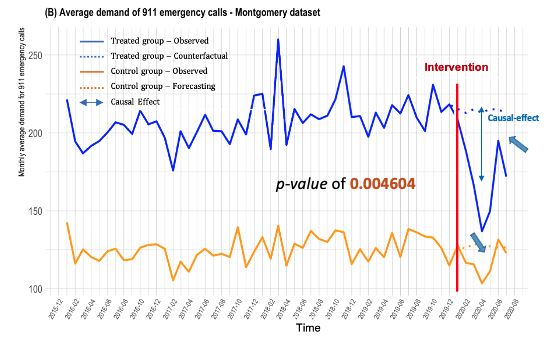
\includegraphics[width=0.80\textwidth]{images/911calls}}
\caption{ \scriptsize The causal effect of the COVID19 lockdown measures over the 911 emergency callouts}
\label{causal}
\end{figure}
\end{frame}


%\begin{frame}{Research Project 4: Publications and Achievements}
%	\small
%\begin{enumerate}
%    \item \textcolor{blue}{Towards Accurate Predictions and Causal `What-if' Analyses for Planning and Policy-making: A Case Study in Emergency Medical Services Demand}\\
%    Authors: Kasun Bandara, Christoph Bergmeir, Sam Campbell, Debbie Scott and Dan Lubman\\
%    Accepted for publication at the \textit{IEEE International Joint Conference on Neural Networks-2020}.
%\end{enumerate}
%\end{frame}


\begin{frame}{Research Project 6}
   \begin{block}{Research Question}	
	Can transfer learning approaches uplift the forecast accuracy of GFMs, in situations where the availability of time series is limited.
	\end{block}
	\begin{itemize}
	\item RNN based GFMs are inherently data ravenous and require significant amount of training data. 
	\vspace{3mm}
		\begin{itemize}
		\item \color{blue} Time series databases are often sparse, and may not hold adequate data.
		\item \color{blue} The GFMs outshine univariate forecasting models, in situations where large quantities of related time series are available.
		\end{itemize}
 \end{itemize}
\end{frame}

\begin{frame}{Research Project 6: Approach}
   \begin{itemize}
	\item A host of transfer learning (TL) schemes to leverage the capabilities of GFMs to generate accurate forecast, in situations with less time series data
	\vspace{1mm}
		\begin{itemize}
		\item \color{blue} Adding residual connections to the RNN architecture.
		\item \color{blue} Inspired by the ResNet architecture used for image classification tasks \cite{He2016-wm}.
		\item \color{blue} Allows to introduce substantially deeper GFM architectures.
 		\end{itemize}
 		\vspace{2mm}
 	\item When TL methodology is constrained by the unavailability of a source dataset ($D_s$) to pre-train a model
 	\begin{itemize}
		\item \color{blue} Using a statistical generative model to artificially generate new copies of time series.
		\item \color{blue} GRATIS package introduced by \cite{Kang2019-dy}.
		\item \color{blue} Employs a mixture autoregressive (MAR) models together with genetic algorithms to generate time series.
 		\end{itemize}
\end{itemize}
\end{frame}

\begin{frame}{Research Contribution 6: Residual RNN Architecture}
   \begin{figure}[htbp]
\centerline{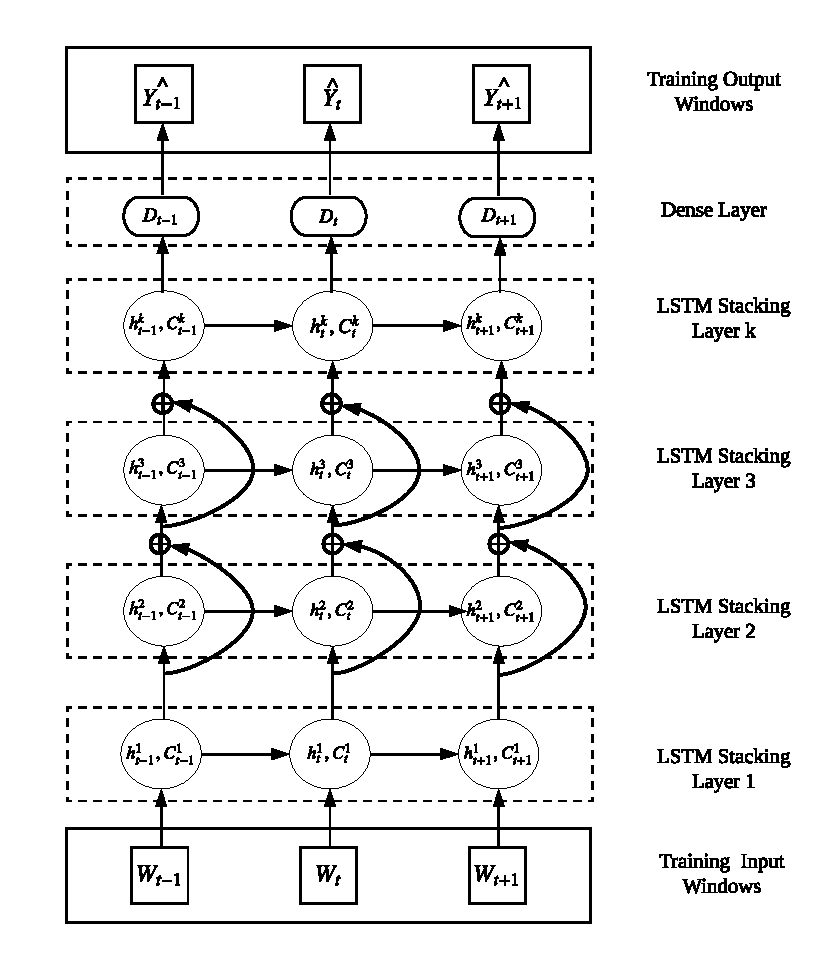
\includegraphics[width=0.42\textwidth]{images/resnetarch}}
\caption{ \tiny The unrolled representation of a residual recurrent network architecture with $k$ number of stacking layers. Here, the residual connections are represented by curved arrows. Accordingly to \cite{He2016-wm}, these residual connections allow the stacking layers to fit a residual mapping between $W_t$ and $\hat{Y_{t}}$, while avoiding the network degradation with network depth increasing}
\label{forecastingarch}
\end{figure}
\end{frame}

\begin{frame}{Research Contribution 6: Overall Architecture }
   \begin{figure}[htbp]
\centerline{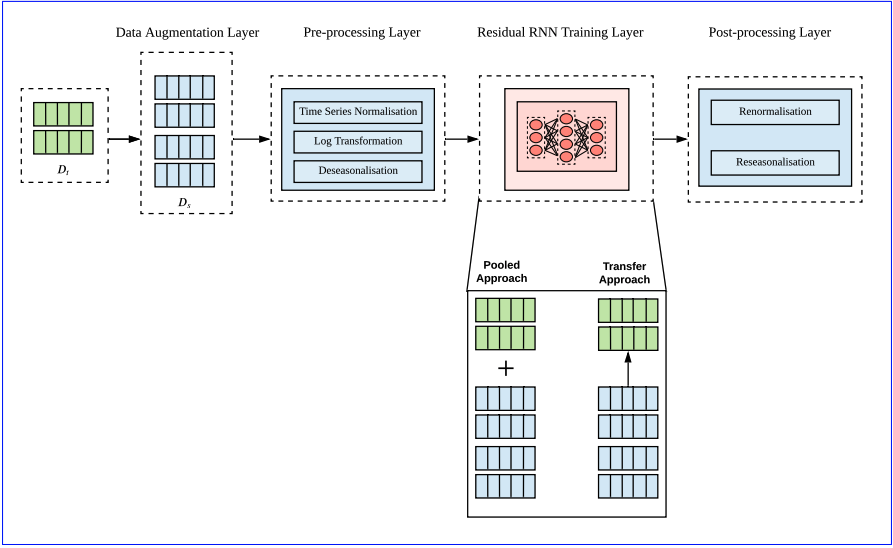
\includegraphics[width=0.65\textwidth]{images/rp5_arch}}
\caption{ \tiny An overview of the proposed framework, which includes a data augmentation layer, pre-processing
layer, residual RNN training layer, and a post-processing layer}
\label{forecastingarch}
\end{figure}
\end{frame}

\begin{frame}{Research Contribution 6: Transfer Learning Architectures}  
\begin{figure}[ht]
\centering
\subfloat[TL-1]{
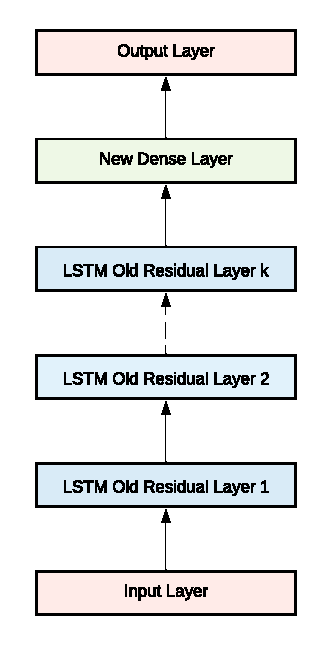
\includegraphics[width=0.15\textwidth]{images/TL1}
\label{fig:subfig1}}%\hfill
\subfloat[TL-2]{
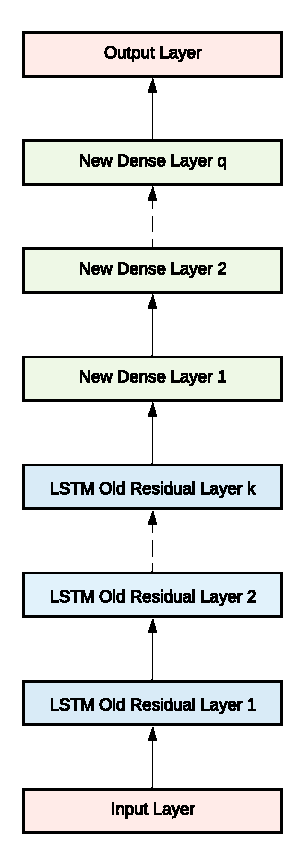
\includegraphics[width=0.15\textwidth]{images/TL2}
\label{fig:subfig2}}%\\[-2ex]
\subfloat[TL-3]{
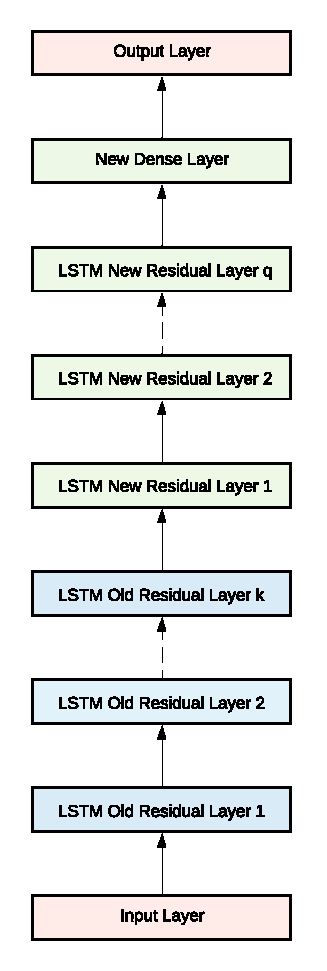
\includegraphics[width=0.15\textwidth]{images/TL3}
\label{fig:subfig3}}%\hfill
\caption{\tiny The layers used to build the base model using the $D_s$, are represented in blue colour, while the additional layers introduced, when building the target model using the $D_t$, are represented in green colour.}
\label{fig:transfarch}
\end{figure}
\end{frame}

% \begin{frame}{Other Projects}
%  \begin{itemize}
%	\vspace{2.0mm}
%	\item Recurrent Neural Networks for Time Series Forecasting: Current Status and Future Directions (Accepted at IJF)
%		\item Causal Inference Using Global Forecasting Models for Counterfactual Prediction (Accepted at PAKDD)
%		\item Global models for time series forecasting: A simulation study (Submitted to Pattern Recognition)
%		\item Ensembles of Localised Models for Time Series Forecasting (Submitted to Data Mining and Knowledge Discovery) 
%		\item The Importance of Environmental Factors in Forecasting Australian Power Demand (Submitted to Environmental Modeling and Assessment)
%		\item An Interpretable Machine Learning Approach to Predicting Customer Behavior on JD. Com
%	\end{itemize}	
%  \end{frame}  
  
%  \begin{frame}{Counterfactual Prediction}
%   \begin{figure}[htbp]
%\centerline{\includegraphics[width=0.80\textwidth]{counter}}
%\caption{ \tiny An example of counterfactual prediction}
%\label{counterfactual}
%\end{figure}
%\end{frame}

\section{Recent Developments}

	\AtBeginSection[]
    {
      \ifnum \value{framenumber}>1
        \begin{frame}<*>
        \frametitle{Outline}
        \begin{minipage}[t]{0.48\textwidth} 
		\end{minipage}
		\begin{minipage}[t][0.6\textheight]{0.50\textwidth}
		 \vspace{0pt} 
 		 \tableofcontents[currentsection]
		\end{minipage}
        
        \end{frame}
      \else
      \fi
    }

  
 \begin{frame}{Current research in GFMs}
  \begin{itemize}
  		\item Global models for hierarchical time series forecasting 
  		\vspace{2mm}
  		\item Interpretable forecasts for global models
  		\vspace{2mm}
  		\item Global models robust to concept drift.
  		\vspace{2mm}
  		\item Global models for scenario-forecasting.
		\end{itemize}
  \end{frame}  


  \begin{frame}
  \begin{center}
  {\Huge Thank you}\vspace{1cm}\\
  Kasun Bandara\vspace{0.2cm}\\
  \textcolor{DiCITSBlue}{Kasun.Bandara@unimelb.edu.au}\vspace{0.2cm}\\
  Slides available: \scriptsize{\url{github.com/kasungayan/GoogleTalk}}
  
  \end{center}
\end{frame}

\begin{frame}[allowframebreaks]{References} 
  \scriptsize
\bibliographystyle{apalike}
\bibliography{reference}
\end{frame}

\begin{frame}{Appendix}
  	\begin{figure}
   
\includegraphics[scale=0.40]{images/trainvalidation}
   \caption{}
  \end{figure} 
\end{frame}


%
%\begin{frame}{Questions}
%\centering
%\begin{figure}
%\includegraphics[scale=0.2]{questions}
%\end{figure}
%\end{frame}





\end{document}
